This is an example on the following auto regressive (AR) process : \[ X_k = 0.8 X_{k-1} + Wk \] where, $ X_{k} \in \mathcal{R} $, $ W_k \sim \mathcal{N}(0,0.1) $ \begin{Desc}
\item[]\end{Desc}
This state is then observed by the output $ Y_k \in \mathcal{R} $ : \[ Y_k = X_k + V_k \] where $ V_k \sim \mathcal{N}(0,1) $\hypertarget{page1_sec1}{}\section{Define the AR model}\label{page1_sec1}
First the ar process must be define as a sister class of \hyperlink{class_gaussian___linear___model}{Gaussian\_\-Linear\_\-Model}. 

\begin{DocInclude}\begin{verbatim}#ifndef __AR_PROCESS
#define __AR_PROCESS

#include <bfilt/gaussian_model.h>

class AR_Process : public Gaussian_Linear_Model
{
public :
      AR_Process(void);
};


#endif
\end{verbatim}
\end{DocInclude}
 The Gaussian Linear \hyperlink{class_model}{Model} are implemented in the following form : \[ X_k = F X_{k-1} + f + G W_k \] \[ Y_k = H X_{k-1} + h + V_k \] The constructor of AR\_\-Process is then : 

\begin{DocInclude}\begin{verbatim}#include "ar_process.h"

AR_Process::AR_Process(void)
{
      // State Equation
      F.resize(1,1);
      F(0,0) = 0.8;

      f.resize(1);
      f(0) = 0.;
      
      G.resize(1,1);
      G.identity();
      
      Qw.resize(1);
      Qw(0,0)= 0.1;

      // Observation noise
      H.resize(1,1);
      H(0,0) = 1;

      h.resize(1);
      h(0) = 0.;

      Qv.resize(1);
      Qv(0,0)=1;
  
      // Init state 
      X0.resize(1);
      X0(0) = 10.;

      R0.resize(1);
      R0.zero();
}
\end{verbatim}
\end{DocInclude}
\hypertarget{page2_sec2}{}\section{The main program}\label{page2_sec2}
In the main program, the model will be first simulted with a specific simulator for gaussian model (\hyperlink{class_g___simulator}{G\_\-Simulator}). Then the simulated output sequence $ y_{0:N}$ is given to the input of a discrete-discrete kalman filter (DD\_\-Filter) to estimate the state $ \hat{X}_{0:k} $. First, all this objects are declared :

 

\begin{DocInclude}\begin{verbatim}int main(int argc, char **argv)
{
      AR_Process model;            // The AR model

      G_Simulator sim(&model);      // The simulator
      
      DD_Kalman  filter(&model);   // The Kalman filter 
\end{verbatim}
\end{DocInclude}


Then 100 samples are simulated : 

\begin{DocInclude}\begin{verbatim}      sim.Simulate(100);
\end{verbatim}
\end{DocInclude}
 The kalman filter is apply on the output sequence : 

\begin{DocInclude}\begin{verbatim}\end{verbatim}
\end{DocInclude}
 You can save the simulated sequences : 

\begin{DocInclude}\begin{verbatim}      sim.Save_Y("output.dat");
      sim.Save_X("state.dat");
\end{verbatim}
\end{DocInclude}


and the estimated state : 

\begin{DocInclude}\begin{verbatim}      filter.Save_X("estimation.dat");
\end{verbatim}
\end{DocInclude}


After compileing and execution, with Gnuplot you can plot : 

\begin{Code}\begin{verbatim}  plot 'state.dat' w l, 'estimation.dat' w l, 'output.dat'
\end{verbatim}
\end{Code}

 To obtain the following graph :  \begin{ImageNoCaption}\mbox{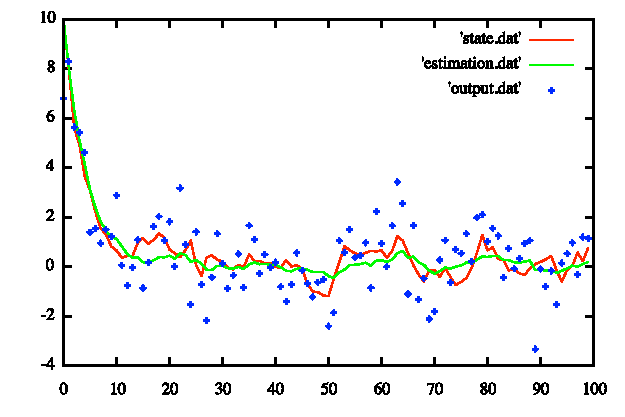
\includegraphics{ar_process}}
\end{ImageNoCaption}
\hypertarget{page2_sec3}{}\section{The CMakeList.txt}\label{page2_sec3}


\begin{DocInclude}\begin{verbatim}CMAKE_MINIMUM_REQUIRED(VERSION 2.6)

PROJECT(Van_Der_Pol)
ADD_DEFINITIONS(" -O3")

# GSL
SET(BFILT_LIB bfilt)

# Include et Link Directories

IF(APPLE)
  MESSAGE("-- Apple Configuration")
  INCLUDE_DIRECTORIES(
    /sw/include/
    )
ENDIF(APPLE)

# Executables and "stand-alone " librairies
ADD_EXECUTABLE (Van_Der_Pol
  van_der_pol.cpp
  example_3.cpp
  )

# Linkage
TARGET_LINK_LIBRARIES(Van_Der_Pol
  ${BFILT_LIB}     
  )
\end{verbatim}
\end{DocInclude}
 